\documentclass{article}
\usepackage[bottom=1cm, top=1cm, left=1cm, right=1cm, paperheight=20cm, paperwidth=20cm]{geometry}
\usepackage{tikz,pgf}
\usetikzlibrary{intersections}

\begin{document}
\pagestyle{empty}

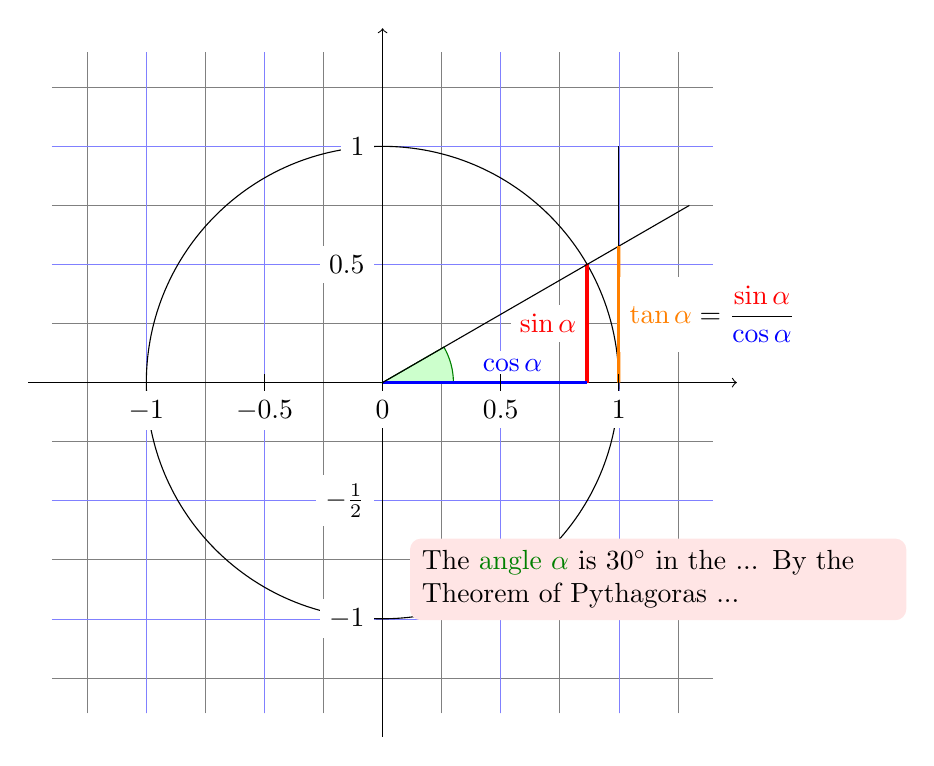
\begin{tikzpicture}[scale=3, 
    information text/.style={rounded corners,fill=red!10,inner sep=1ex}] 
    %\clip (-2,-2) rectangle (2, 2);
    \tikzset{help lines/.style={color=blue!50,very thin}};
    \draw[step=0.25cm, gray, very thin] (-1.4, -1.4) grid (1.4, 1.4);
    \draw[step=0.5cm, help lines] (-1.4, -1.4) grid (1.4, 1.4);
    \draw[->] (-1.5,0) -- (1.5,0);
    \draw[->] (0,-1.5) -- (0,1.5);
    \draw (0,0) circle (1cm);
    %\draw (3mm,0mm) arc (0:30:3mm);
    \filldraw[fill=green!20!white, draw=green!50!black] (0,0) -- (3mm, 0mm) arc (0:30:3mm) -- cycle;
    \draw[color=red, very thick] (30:1) -- node[fill=white, anchor=east] {$\sin\alpha$} +(0, -0.5);
    \draw[color=blue, very thick] (30:1) ++(0,-0.5) -- node[above, xshift=10pt, fill=white] {$\cos\alpha$} (0, 0);
    \draw[name path=upward line] (1,0) -- (1,1);
    \draw[name path=sloped line] (0,0) -- (30:1.5cm);

    \draw[name intersections={of=upward line and sloped line, by=x}][very thick, orange] (1,0) -- node[anchor=west, fill=white] {$\displaystyle \tan\alpha \color{black}= \frac{\color{red}\sin\alpha}{\color{blue}\cos\alpha}$} (x);

    \foreach \x in {-1, -0.5, ..., 1} 
        \draw (\x cm, 1pt) -- (\x cm, -1pt) node[anchor=north, fill=white] {$\x$};
    %\foreach \x in {-1, -0.5, ..., 1} 
    %    \draw (-1pt, \x cm) -- (-1pt, \x cm) node[anchor=east] {$\x$};
    
    \foreach \x/\xtext in {-1, -0.5/-\frac{1}{2}, 0.5, 1} 
        \draw (-1pt, \x cm) -- (-1pt, \x cm) node[anchor=east, fill=white] {$\xtext$};

    \draw (1, -1) node[xshift=0.5cm, yshift=0.5cm, text width=6cm, information text]
        {
            The {\color{green!50!black} angle $\alpha$} is $30^\circ$ in the ... By the Theorem of Pythagoras ...
        };
\end{tikzpicture}
\end{document}
